\documentclass[17pt, aspectratio=169]{beamer}

\beamertemplatenavigationsymbolsempty
\usetheme{CambridgeUS}
\usecolortheme{dolphin}
\useinnertheme{rectangles}
\usepackage{array}
\usepackage[subpreambles=true]{standalone}
\usepackage{import}


\title{M.O.S.I.S Final Report Presentation}
\author[Fabio J. \& Eduardo S.]{Fabio J. Matos Nieves \& Eduardo S. Miranda Figueroa}
\institute[UPRM]{University of Puerto Rico Mayagüez Campus}
\date{December 11, 2023}

\begin{document}
\begin{frame}
	\maketitle
\end{frame}
\begin{frame}{Agenda}
	\tableofcontents
\end{frame}
\section{Introduction}
\subsection*{Background}
\begin{frame}{What is M.O.S.I.S?}
	\begin{columns}
		\column{0.5\textwidth}
		\centering
		\textbf{M.O.S.I.S}\\
		Marine Operated Stereoscopic Imaging System

		\column{0.5\textwidth}
		\centering
		\begin{figure}
			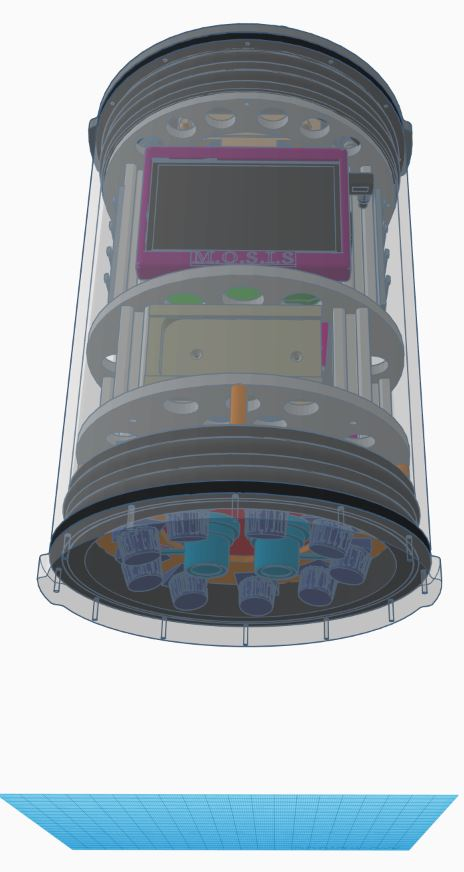
\includegraphics[height=0.85\textheight]{./Figures/M.O.S.I.S_Model.jpeg}
		\end{figure}
	\end{columns}
\end{frame}
\begin{frame}{What is the problem?}
	\begin{itemize}
		\item The M.O.S.I.S microscope already had a user interface \textbf{but}:
		      \begin{itemize}
			      \item lacked design cohesion.
			      \item had missing and redundant features.
			      \item constantly crashes.
			      \item lacked a formal way to store data.
		      \end{itemize}
	\end{itemize}
\end{frame}
\subsection*{Deliverables and Milestones}
\begin{frame}{Deliverables}
	\begin{itemize}
		\item User interface for the M.O.S.I.S microscope that can:
		      \begin{itemize}
			      \item display the live feed for both cameras and sensor data.
			      \item capture single, burst, time lapse and telescopic images plus video.
			      \item utilize the on board buttons for navigation.
			      \item control the on board lighting and camera settings.
			      \item calibrate pH and dissolved oxygen sensors
		      \end{itemize}
	\end{itemize}

\end{frame}
\begin{frame}{Milestones}
	\begin{center}
		\begin{tabular}{||c | c||}
			\hline
			Back end API               & Oct 15, 2023 \\
			\hline
			Front end                  & Oct 24, 2023 \\
			\hline
			Folder Structure Generator & Oct 26, 2023 \\
			\hline
			Hardware API + Integration & Nov 27, 2023 \\
			\hline
		\end{tabular}
	\end{center}
\end{frame}
\subsection*{Expenditure Summary}
\begin{frame}{Expenditure Summary}
	\begin{center}
		\textbf{Total Estimated Cost}
		\begin{tabular}{||m{0.75\textwidth}|m{0.20\textwidth}||}
			\hline
			Category             & Cost        \\
			\hline
			Human Resources      & \$18,430.61 \\
			\hline
			Equipment            & \$7,961.98  \\
			\hline
			Facility             & \$1,410.00  \\
			\hline
			Overhead             & \$13,901.01 \\
			\hline
			Total Estimated Cost & \$41,703.03 \\
			\hline
		\end{tabular}
	\end{center}
\end{frame}
\begin{frame}
	\begin{center}
		\textbf{Total Actual Cost}
		\begin{tabular}{||m{0.75\textwidth}|m{0.20\textwidth}||}
			\hline
			Category          & Cost                      \\
			\hline
			Human Resources   & \$18,430.61               \\
			\hline
			Equipment         & \textcolor{teal}{\$29.98} \\
			\hline
			Facility          & \$1,410.00                \\
			\hline
			Overhead          & \$13,901.01               \\
			\hline
			Total Actual Cost & \$33,771.60               \\
			\hline
		\end{tabular}
	\end{center}
\end{frame}
\section{Body}
\subsection*{System Specifications}
\begin{frame}{System Specifications: Hardware}
	\begin{itemize}
		\item 2 PixeLink PL-D755 Cameras
		\item 8 Hall Effect sensor as buttons
		\item 800$\times$480 resolution display
		\item Red, White and Ultraviolet Lighting
		\item Raspberry Pi
	\end{itemize}
\end{frame}
\begin{frame}{System Specifications: Software}
	\begin{itemize}
		\item 400$\times$400 resolution preview for left and right cameras
		\item Displays temperature, pressure, dissolved oxygen and pH sensor data
		\item User interface utilizes on board buttons
		\item Controls camera parameters and on board lighting
		\item Calibrates pH and dissolved oxygen sensors
		\item Written in Python using PyQt6 and SQLite3
	\end{itemize}
\end{frame}
\subsection*{Validation and Testing}
\begin{frame}{Validation}
	\begin{enumerate}
		\item Thorough review of the system requirements
		\item Constant feedback from the client and stakeholder
	\end{enumerate}
\end{frame}
\begin{frame}{Testing}
	\begin{enumerate}
		\item Module Testing
		\item Integration Testing
		\item End to end testing
	\end{enumerate}
\end{frame}
\subsection*{Design Alternatives}
\begin{frame}{Design Alternatives}
	\begin{itemize}
		\item There are three main architectural patterns used to create user interfaces
		      \begin{enumerate}
			      \item Web based
			      \item Native
			      \item Web-Native
		      \end{enumerate}
	\end{itemize}
\end{frame}
\begin{frame}{Software Alternatives}
	\begin{itemize}
		\item Main programming Language: Python
		\item Desire for free and open source software
		      \begin{itemize}
			      \item User interface library from scratch
			      \item PyQt6
			      \item PyGTK
		      \end{itemize}
	\end{itemize}
\end{frame}
\subsection*{Diagrams}
\begin{frame}{M.O.S.I.S UI 2.0: System Architecture}
	\begin{figure}
		\resizebox{\textwidth}{!}{
			\begin{small}
				\import{./Figures}{system_architecture}
			\end{small}
		}
		\caption{System Architecture}
	\end{figure}
\end{frame}
\subsection*{Pictures}
\begin{frame}{M.O.S.I.S UI 2.0: System Architecture}
	\begin{figure}
		\resizebox{!}{0.65\textheight}{
			\begin{small}
				\import{./Figures}{hardware_interfaces}
			\end{small}
		}
		\caption{System Architecture: Hardware Interfaces}
	\end{figure}
\end{frame}
\begin{frame}
	\textbf{M.O.S.I.S Microscope}
	\begin{figure}
		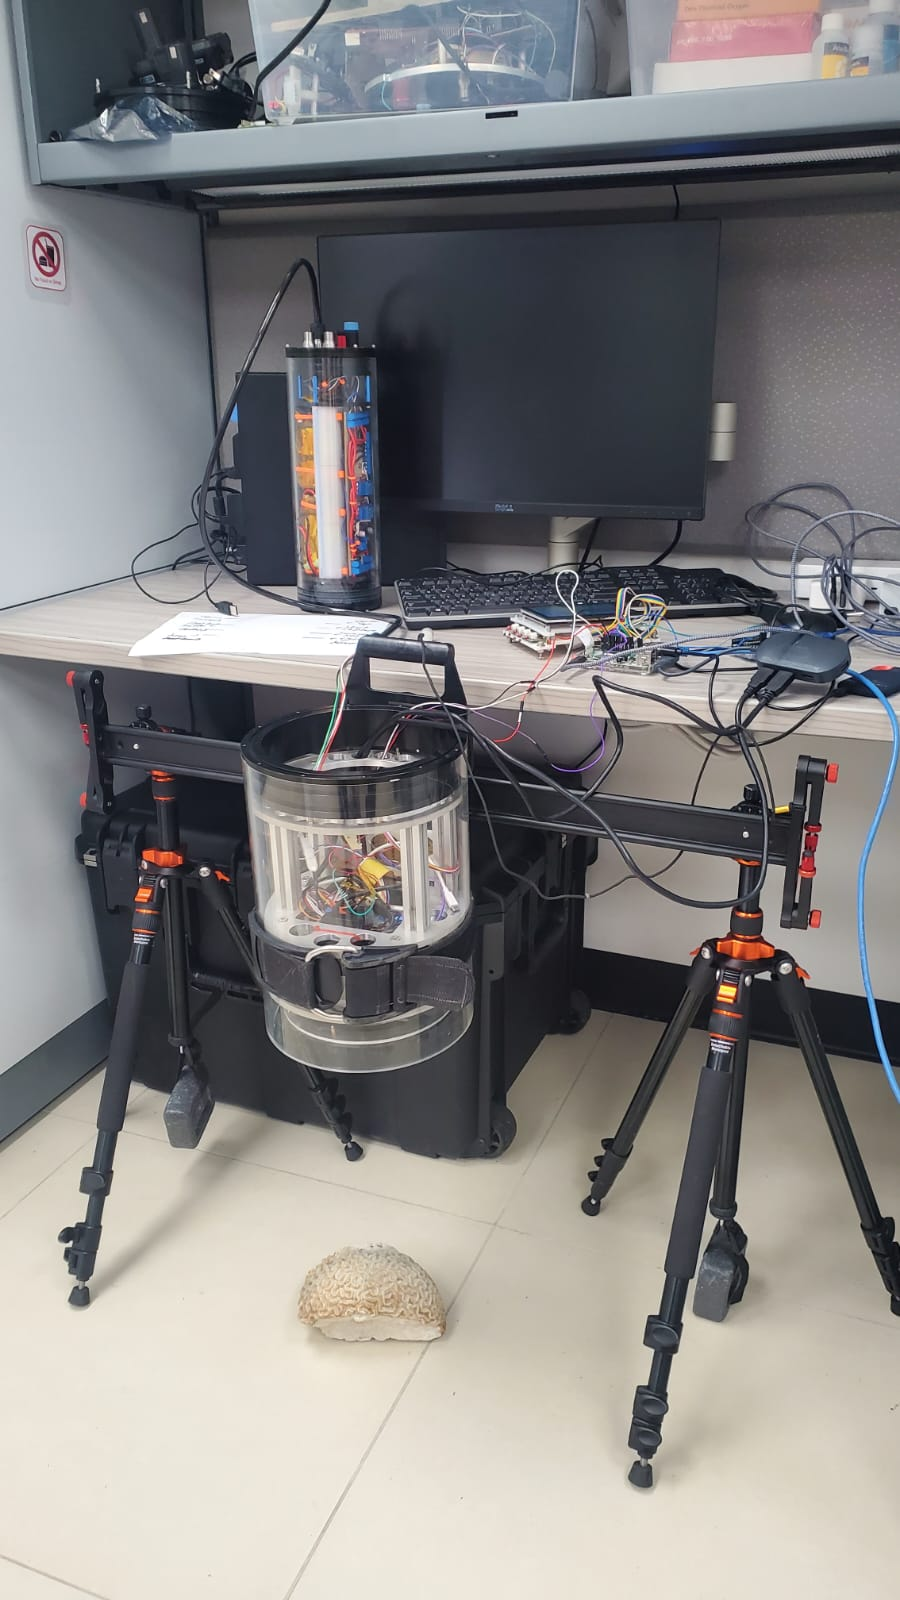
\includegraphics[width=\textwidth, height=\textheight, keepaspectratio]{./Figures/MOSIS.jpg}
		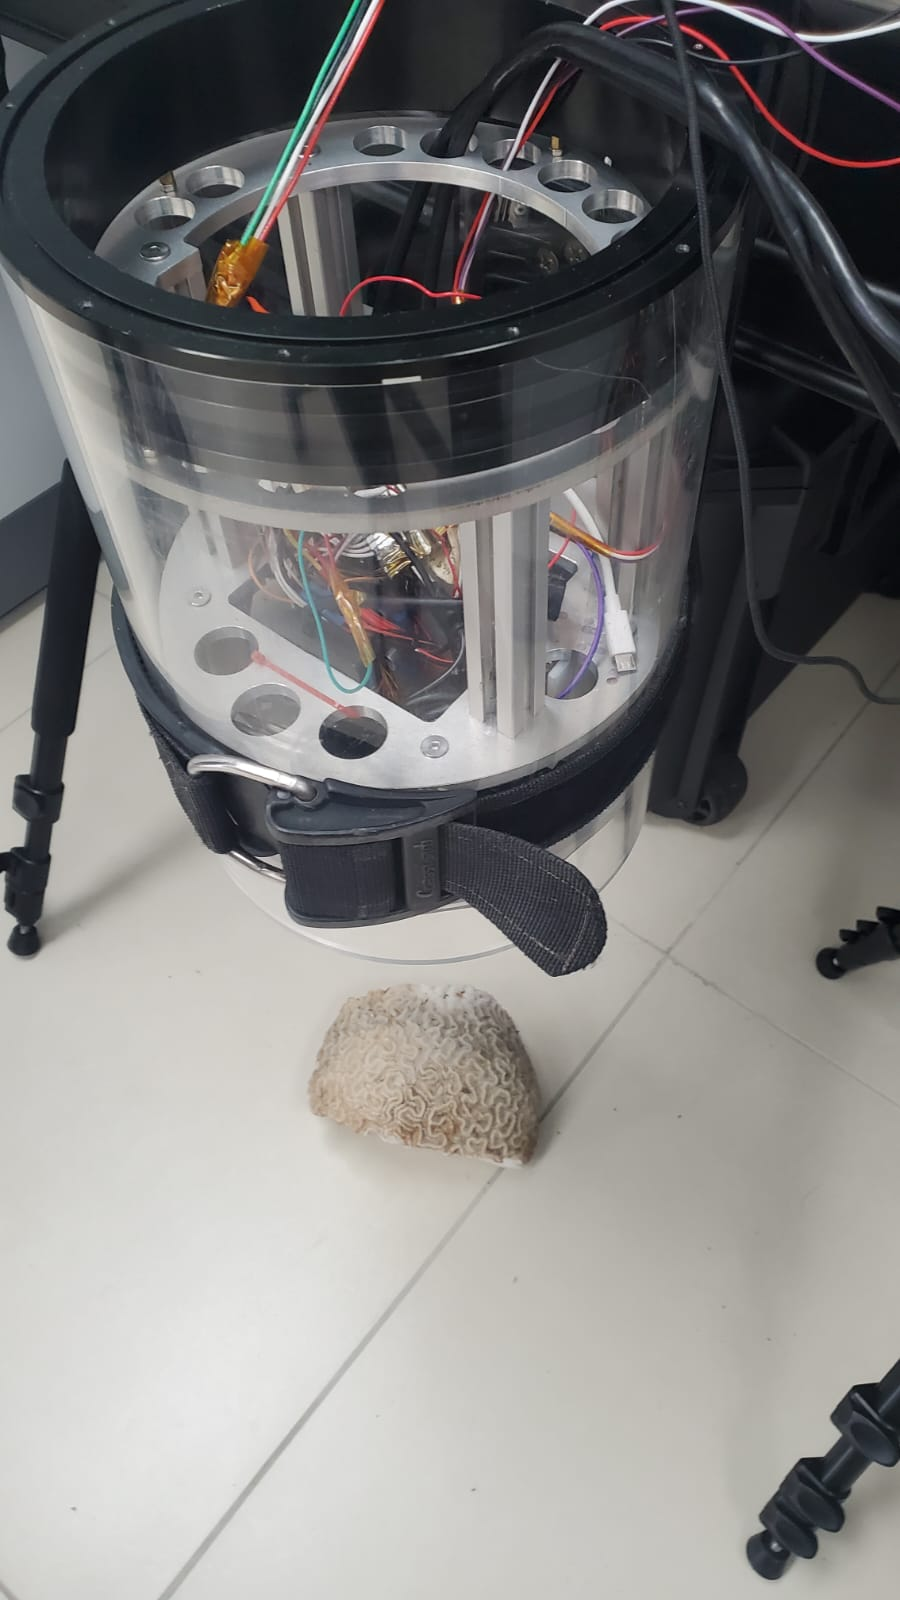
\includegraphics[width=\textwidth, height=\textheight, keepaspectratio]{./Figures/MOSIS2.png}
	\end{figure}
\end{frame}
\begin{frame}
	\textbf{Telescopic Image Example}
	\begin{figure}
		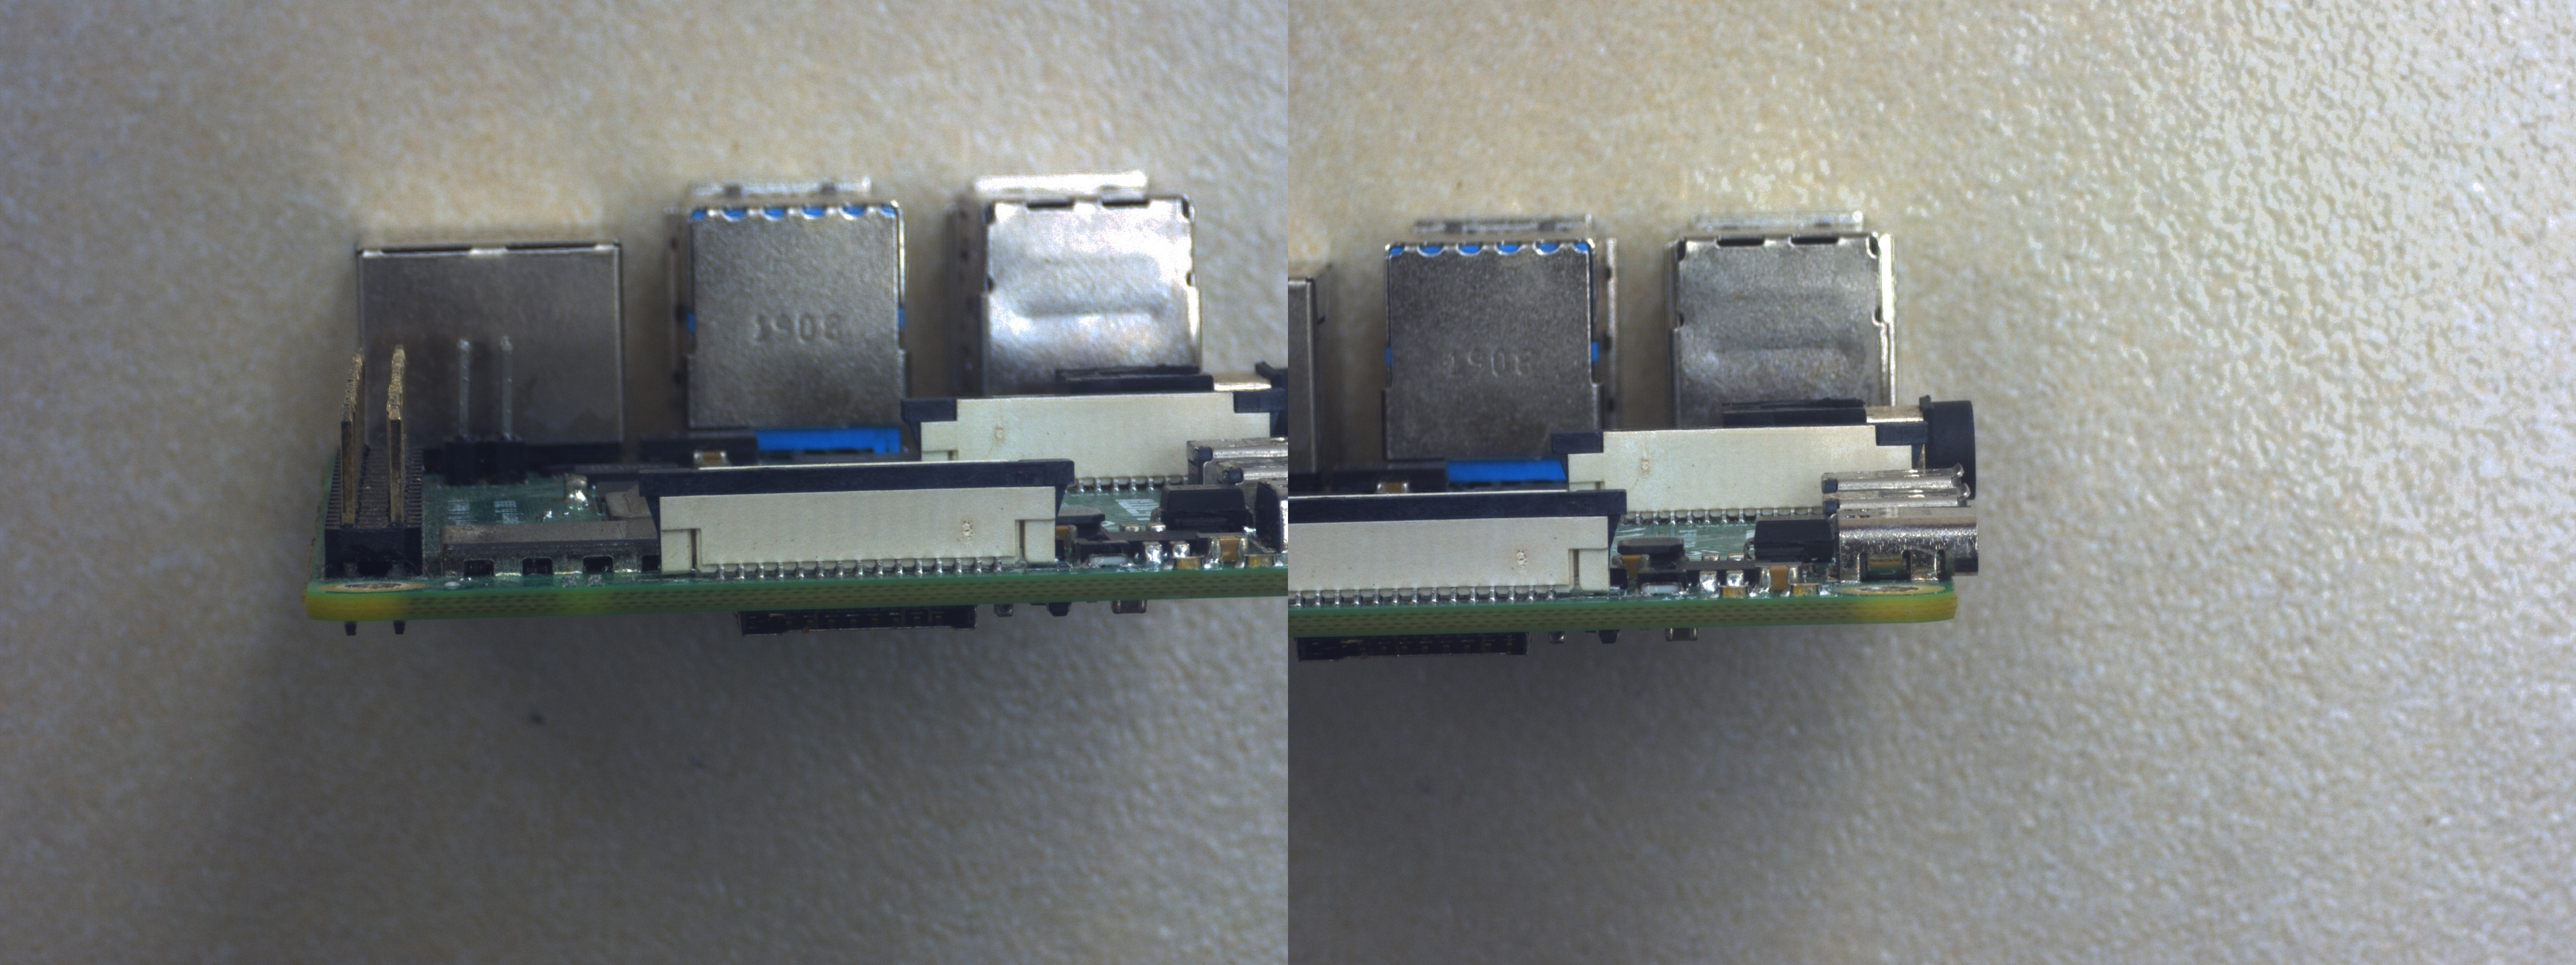
\includegraphics[width=\textwidth, height=\textheight, keepaspectratio]{./Figures/focusStack-S.jpg}
	\end{figure}
\end{frame}
\subsection{Video Demo}
\begin{frame}{Video Demonstration}
	\href{https://youtu.be/JZFvu8QhQfI}{Video Link}
\end{frame}
\subsection{Project Assessment}
\begin{frame}{Project Assessment}
	\begin{itemize}
		\item Positives
		      \begin{itemize}
			      \item Completed integration for the M.O.S.I.S microscope's hardware modules
			      \item Progressed the M.O.S.I.S microscope project from just a preview screen to a functional prototype
			      \item The microscope can now be utilized in the field
		      \end{itemize}
		\item Negatives
		      \begin{itemize}
			      \item The current user interface suffers from low responsiveness
		      \end{itemize}
	\end{itemize}
\end{frame}
\subsection*{Project Impact}
\begin{frame}{Project Impact}
	\begin{itemize}
		\item The microscope can now be used in the study the effects of ocean acidification on coral reefs.
		      \begin{itemize}
			      \item Hasten environmental research
			      \item Record environmental conditions
			      \item Perform various kinds of studies quickly and efficiently.
		      \end{itemize}
		\item Subsequent research can inform the public on the effects of climate change.
	\end{itemize}
\end{frame}
\section{Conclusion}
\subsection{Project Summary}
\begin{frame}{Project Summary}
	\begin{itemize}
		\item Created a fully functional user interface for the M.O.S.I.S microscope
		\item Integrated all hardware for the microscope
		\item The project can now be used in the field to produce environmental research
	\end{itemize}
\end{frame}
\subsection{Difficulties}
\begin{frame}
	\begin{itemize}
		\item Poor documentation
		      \begin{itemize}
			      \item Camera software development kit (SDK)
			      \item Existing camera functions
		      \end{itemize}
		\item Camera SDK has missing features on Raspberry Pi OS
	\end{itemize}
\end{frame}
\subsection{Achievements and Lessons Learned}
\begin{frame}{Lessons Learned and Achievements}
	\begin{itemize}
		\item The importance of:
		      \begin{itemize}
			      \item Teamwork and cooperation
			      \item Prior experience in project management
			      \item Thorough planning and documentation
			      \item being able to communicate with people in and out of your field of expertise
		      \end{itemize}
		\item Contributed in climate research
		\item Gained experience as a designer and consultant
	\end{itemize}
\end{frame}
\subsection{Future Work}
\begin{frame}{Future Work}
	\begin{itemize}
		\item Increase frame rate of the camera preview
		\item On screen display for button controls
		\item Brightness control on lighting
		\item Camera auto focus
		\item Focus point visualizer
	\end{itemize}
\end{frame}
\subsection{Questions}
\begin{frame}
	Questions?
\end{frame}
\end{document}